% Source of the figure transition-graph.pdf (transitions between the paths of the chain links, by link type).
% Compile with pdfLaTeX; the PDF is included in the manuscript at its natural size.
\documentclass[tikz,border=1pt]{standalone}
\usepackage[T1]{fontenc}
\usepackage{stix}
\pdfinfoomitdate=1 \pdftrailerid{} \pdfsuppressptexinfo=-1
\begin{document}
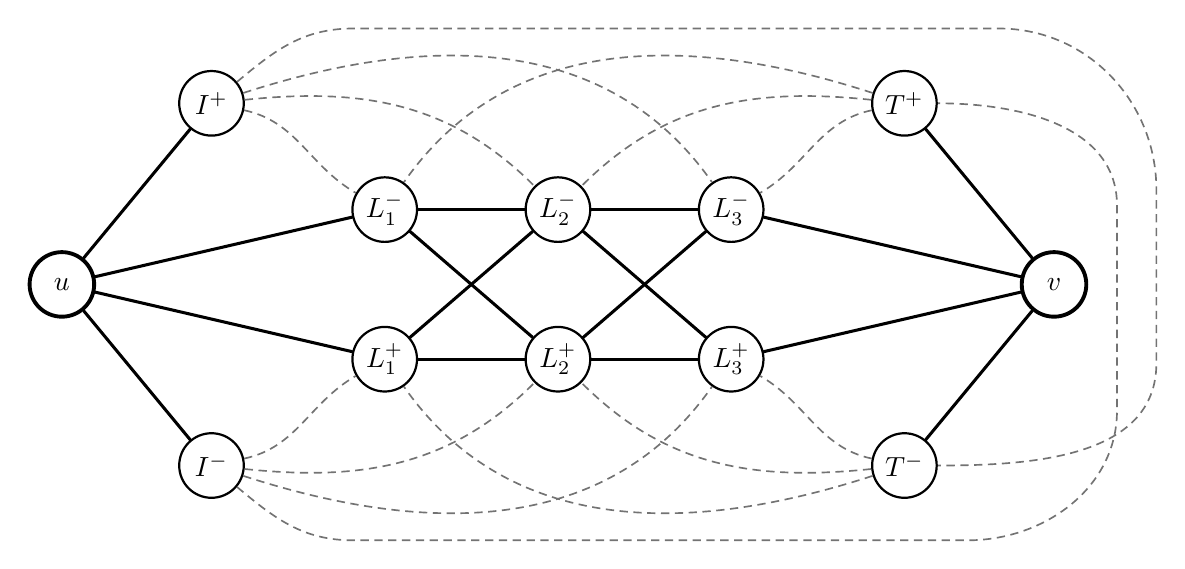
\begin{tikzpicture}[x=1cm, y=1cm,
    vertex/.style={circle, draw, line width=0.8pt, inner sep=0pt, minimum size=0.82cm},
    terminal/.style={vertex, line width=1.4pt},
    stays/.style={line width=1.1pt, line cap=round},
    vanishes/.style={line width=0.6pt, densely dashed, black!55}]
  % u, v and one vertex for each path of a chain link; the negative paths of the literal links are drawn in
  % the upper row, next to the positive paths of the initialization and terminal links they are joined to.
  \node[terminal] (u)  at (-6.3, 0)   {$u$};
  \node[terminal] (v)  at ( 6.3, 0)   {$v$};
  \node[vertex]   (Ip) at (-4.4, 2.3) {$I^{+}$};
  \node[vertex]   (Im) at (-4.4,-2.3) {$I^{-}$};
  \node[vertex]   (Tp) at ( 4.4, 2.3) {$T^{+}$};
  \node[vertex]   (Tm) at ( 4.4,-2.3) {$T^{-}$};
  \foreach \j/\x in {1/-2.2, 2/0, 3/2.2} {
    \node[vertex] (L\j m) at (\x, 0.95) {$L_{\j}^{-}$};
    \node[vertex] (L\j p) at (\x,-0.95) {$L_{\j}^{+}$};}

  % synchronization threads, between two chain links of a block: opposite signs; the two edges between
  % the initialization and the terminal link run around the drawing
  \draw[vanishes] (Ip) to[out=40, in=180] (-2.6,3.25) -- (5.6,3.25) to[out=0, in=90] (7.6,1.2) -- (7.6,-1.0)
                       to[out=-90, in=0] (Tm);
  \draw[vanishes] (Im) to[out=-40, in=180] (-2.6,-3.25) -- (5.2,-3.25) to[out=0, in=-90] (7.1,-1.6) -- (7.1,1.0)
                       to[out=90, in=0] (Tp);
  \draw[vanishes] (Ip) to[out=-12, in=150]  (L1m);
  \draw[vanishes] (Ip) to[out=6,   in=135]  (L2m);
  \draw[vanishes] (Ip) to[out=18,  in=125]  (L3m);
  \draw[vanishes] (Tp) to[out=192, in=30]   (L3m);
  \draw[vanishes] (Tp) to[out=174, in=45]   (L2m);
  \draw[vanishes] (Tp) to[out=162, in=55]   (L1m);
  \draw[vanishes] (Im) to[out=12,  in=-150] (L1p);
  \draw[vanishes] (Im) to[out=-6,  in=-135] (L2p);
  \draw[vanishes] (Im) to[out=-18, in=-125] (L3p);
  \draw[vanishes] (Tm) to[out=168, in=-30]  (L3p);
  \draw[vanishes] (Tm) to[out=186, in=-45]  (L2p);
  \draw[vanishes] (Tm) to[out=198, in=-55]  (L1p);

  % synchronization threads at u and v
  \draw[stays] (u) -- (Ip);
  \draw[stays] (u) -- (Im);
  \draw[stays] (Tp) -- (v);
  \draw[stays] (Tm) -- (v);
  % clause threads
  \draw[stays] (u) -- (L1m);
  \draw[stays] (u) -- (L1p);
  \draw[stays] (L3m) -- (v);
  \draw[stays] (L3p) -- (v);
  \foreach \a/\b in {1/2, 2/3} {
    \draw[stays] (L\a m) -- (L\b m);
    \draw[stays] (L\a p) -- (L\b p);
    \draw[stays] (L\a m) -- (L\b p);
    \draw[stays] (L\a p) -- (L\b m);}
\end{tikzpicture}
\end{document}
